% paper_draft.tex — MazeWeb Paper v0.5 (重写: 真实 grid 截图 + 中文摘要 + 修配色)
% sko (冯卓源)
% 编译: xelatex paper_draft.tex (2 轮)
%
% 关键改动 (vs v0.4):
%   - 摘要改中文
%   - 删 self-reference 命名 (M4 SOTA / M5 等中间词)
%   - 真实 WebGPU 渲染的 CA grid 截图替代 Python 重现 (manhattan-2/chebyshev-1/2/4/manhattan-1/4)
%   - Spiral 修对 (同心螺旋通道, 不是实心填充)
%   - sweep 4-panel 用 ndjson 真实数据
%   - 配色统一暖纸 + 朱红 + 墨黑 (印刷友好, 无彩虹)
%
% 数据:
%   - sweep_2026_07_04/results.ndjson (128 runs, 122 OK)
%   - ckpt/  (122 bestChromBits JSON)
%   - preview tab 截图 (figures/v2/grid_*.png) — 浏览器 WebGPU 实际渲染
%   - _gen_grids.mjs 脚本生成 6 真迷宫 + 9 伪迷宫 (Spiral 已修)

\documentclass[11pt,a4paper]{article}

\usepackage[UTF8,fontset=windows]{ctex}
\usepackage[a4paper,margin=2.2cm]{geometry}
\usepackage{xcolor}
\usepackage{amsmath,amssymb}
\usepackage{graphicx}
\usepackage{booktabs}
\usepackage{array}
\usepackage{enumitem}
\usepackage{hyperref}
\usepackage{caption}
\usepackage{float}
\usepackage{longtable}
\usepackage{multicol}
\usepackage{multirow}
\usepackage{tikz}
\usepackage{placeins}
\usetikzlibrary{decorations.pathreplacing,calc}
\usepackage{tcolorbox}
\tcbuselibrary{skins,breakable}

% ============ 配色: 暖纸 + 墨黑 + 朱红 (单一克制, 不用彩虹) ============
\definecolor{PaperWarm}{HTML}{F4EAD8}
\definecolor{InkWarm}{HTML}{2C1F17}
\definecolor{Vermilion}{HTML}{B8412F}
\definecolor{OliveWarm}{HTML}{6B7A5C}
\definecolor{GrayMid}{HTML}{7A6A58}
\definecolor{GrayLight}{HTML}{A89888}
\definecolor{SepiaLine}{HTML}{8A6A3A}

\hypersetup{
  colorlinks=true,
  linkcolor=InkWarm,
  citecolor=InkWarm,
  urlcolor=Vermilion,
  pdftitle={FamilyMask: Multi-Family Cellular Automaton Encoding with an 8-Dimensional Maze Quality Metric},
}

% Caption 样式: 小字 + Vermilion label
\captionsetup{labelfont={small,bf,color=Vermilion},textfont={small,color=InkWarm},
              labelsep=period,font=small}

% 行距
\linespread{1.18}

% ============ TikZ 染色块 (用同一调色) ============
\newcommand{\cin}{Vermilion}
\newcommand{\oli}{OliveWarm}
\newcommand{\ink}{InkWarm}

\begin{document}

% ============ 标题 ============
\begin{center}
{\Large\bfseries\color{\ink} 多族元胞自动机编码与八维迷宫质量度量}\\[0.3em]
{\large\color{GrayMid} Multi-Family Cellular Automaton Encoding with an\\ Eight-Dimensional Maze Quality Metric}\\[0.6em]
{\small\scshape FamilyMask / maze\_quality (maze-web, July 2026)}\\[0.3em]
{\color{GrayMid}\small sko (冯卓源)\quad$\cdot$\quad 编译于 2026-07-06}
\end{center}

\vspace{0.4em}
\hrule height 0.4pt
\vspace{1.0em}

% ============ 中文摘要 ============
\begin{tcolorbox}[colback=PaperWarm,colframe=SepiaLine,arc=2pt,boxrule=0.5pt,
                  left=10pt,right=10pt,top=8pt,bottom=8pt]
\noindent\textbf{\color{\cin}摘要.}\quad
针对元胞自动机生成的二值图是否为迷宫这一判定难题,本文提出两件互补的产物。
其一,\textbf{FamilyMask}:一种多族染色体编码,把 B/S 型生命周期规则推广为多族组合。
每族独立持有自己的邻域 mask(可达 chebyshev-4 即 $9\times 9$ 中心外 80 格)、出生集、存活集与优先级;
最多十六族并行,执行时按优先级顺序,首个匹配的族决定下一态。
其二,\textbf{maze\_quality}:一种八维几何质量度量,在五个拓扑子度量
(走廊主导度、最长路径占比、十字口占比、最大连通分量占比、外圈抑制) 与
三个多样性子度量(2$\times$2 块熵、镜像不对称度、2$\times$2 邻接对熵) 上做两层加权几何聚合,
并乘以一道在 $[0.30, 0.45]$ 上呈三角形的墙比软门控。
此度量在 15 个对照样本 (六个经典迷宫生成算法 + 九个非迷宫吸引子) 上,
真正迷宫均值 0.707、伪迷宫均值 0.000、间隔 0.707,无误判;
Bellot 2021 的 $F$ 度量在同一数据集上间隔为 $-0.183$,方向相反。

将 FamilyMask 嵌入 200 $\times$ 500 的 $(\mu+\lambda)$ 进化策略,
在 122 次运行 (8 种距离模板 $\times$ 4 个最大族数 $\times$ 4 个随机种子,
40$\times$60 网格, 300 步演化, WebGPU 加速) 上获得最高分 0.8233
(manhattan-2 模板、8 族容量上限、随机种子 444)。
结果显示,
(1) 多族容量上限的提升主要价值在于``偶尔突破''单族天花板,均值并不随之单调上升;
(2) chebyshev-4 模板的均值仅 0.157,主因并非模板无解,而是
其 $9\times 9$ 邻域的染色体搜索空间 ($2^{824}$ 候选)
远大于 ES 在 $10^5$ 次评估预算内可跨越的初始化距离;
(3) manhattan-1 模板的均值仅 0.420,主因是 4 邻域本身无法给元胞提供足够的空间上下文
以涌现走廊结构。
所有实验数据与代码已开源。
\end{tcolorbox}

\vspace{0.8em}

% ============ English Abstract ============
\noindent\textbf{\color{\cin}Abstract.}\quad
We introduce two complementary contributions for evaluating
whether binary grids generated by cellular automata (CA) constitute mazes.
\textbf{FamilyMask} generalises Conway-style life rules to a multi-family chromosome:
each of up to sixteen families owns its own neighbourhood mask (up to a $9\times 9$
centred footprint, 80 cells), birth set, survival set, and priority;
at each step the CA scans active families in priority order and the first match
decides the next cell state.
\textbf{maze\_quality} is an eight-dimensional geometric score aggregating
five topology sub-metrics (corridor dominance, longest-path share, junction share,
largest-component share, outer-frame penalty) and three diversity sub-metrics
($2\times 2$ patch entropy, mirror asymmetry, $2\times 2$ pair entropy) via a
two-level weighted geometric mean, multiplied by a triangular wall-ratio gate
centered at $[0.30,\,0.45]$.
On a 15-pattern benchmark (six classical maze generators plus nine non-maze
attractors) the score attains mean $0.707$ on true mazes and $0.000$ on
pseudo-mazes (gap $+0.707$, zero misclassifications); the Bellot 2021 $F$ score
on the same dataset has gap $-0.183$, with the wrong sign.

Plugging FamilyMask into a 200-population, 500-generation $(\mu+\lambda)$
evolution strategy and running 122 ES sweeps over 8 distance templates,
4 family caps, and 4 random seeds (40$\times$60 grids, 300 CA steps,
WebGPU-accelerated) yields a top score of $0.8233$ (manhattan-2, 8-family
cap, seed 444). We find that (i) larger family caps help mainly by enabling
occasional breakthroughs past the single-family ceiling, not by raising the
mean; (ii) chebyshev-4's poor mean ($0.157$) is not caused by absence of
solutions --- its $9\times 9$ neighbourhood implies a $2^{824}$ candidate
space far beyond the random-init-to-optimum distance $10^5$ ES evaluations can
cross; (iii) manhattan-1's poor mean ($0.420$) is caused by the 4-neighbour
topology providing too little spatial context for corridor emergence.
All code, data, and figures are released as open source.

\vspace{1.2em}

% ============ 1. 引言 ============
\section{引言}
元胞自动机能否生成迷宫,这道问题在 Conway 时代就被反复提出。
早期工作 (Conway 1970; Wolfram 2002 \textit{A New Kind of Science}, ch.\ 6--9)
记录了一千余条规则的演化轨迹,其中若干最终态确实呈迷宫状,
但作者承认选择过程依赖人眼判断,没有可量化的判定准则。
近十年,随着生成式模型与神经 CA 的兴起 (Mordvintsev \textit{et al.} 2020;
Palm \textit{et al.} 2022),CA 再次成为程序化内容生成的工具,
可量化的``是迷宫''判定随之成为瓶颈。

已有的两种判定思路各有局限。
其一,Bellot 2021 提出的 $F$ 度量从迷宫图提取连接性、交叉口计数与回路比例等特征,
与参考真迷宫做加权比较;该度量在多数真迷宫上得分稳定,
但在螺旋、条纹、同心圆等具有``单一贯穿长路径''的几何反例上,
因 F 度量对此结构反而给高分而误判。
其二,Pech 2002 与 Rejbrand 2017 提出在生成阶段直接约束路径结构
(强制单连通、强制 T 形分叉比例) ;这类硬约束对生成器有强侵入性,
难以移植到 CA 这类没有显式构造步骤的演化系统。

本文绕开这两个方向。
\textbf{第一条线}是把 B/S 型规则推广为\textbf{多族组合} (FamilyMask) ,
族之间用优先级仲裁,使搜索空间从单条 B/S 字符串 ($2^{18}$ 候选)
跃升到一族 B/S 加一组 mask ($2^{824}$ 候选),为更复杂的涌现留出余地。
\textbf{第二条线}是提出\textbf{八维几何质量度量} (maze\_quality) ,
子度量全部连续可微 (取值 $[0,1]$,ES 可学),二层加权几何聚合避免单边 exploit,
并用一道墙比软门控拦截 ``实心块'' 与 ``空盒'' 两种典型病态吸引子。
此度量与 Bellot $F$ 在同一 15-pattern 数据集上方向相反:
maze\_quality 真假间隔 $+0.707$ (正向),$F$ 真假间隔 $-0.183$ (反向)。

把 FamilyMask 与 maze\_quality 联立,放进 WebGPU 加速的 $(\mu+\lambda)$ ES,
在 122 次 sweep 上得到 0.8233 的最高分 (manhattan-2 / 8 族 / 种子 444) ,
并从失败样本中分离出两类机制截然不同的病态:
\textbf{搜索空间过大} (chebyshev-4, $0.157$) 与
\textbf{邻域信息不足} (manhattan-1, $0.420$) 。

% ============ 2. 相关工作 ============
\section{相关工作}
\textbf{CA 与迷宫生成.}
Conway 1970 在生命游戏中观察到 ``滑翔机'' 与 ``滑翔机枪'',
Wolfram 2002 在其专著中系统分类了基本 CA 在多初始下的终态,
其中偶见迷宫状吸引子。
Mitchell \textit{et al.} 1993 用遗传算法搜索 CA 密度分类规则,
展示了``计算涌现''在简单规则集中的可行性,
但其目标函数 (密度分类准确率) 与迷宫结构无直接关联。

\textbf{迷宫质量度量.}
Bellot 2021 提出基于路径计数与回路比例的 $F$ 度量,
被 MazeBench 用作多生成器对比基准;
Pech 2002 建议通过 ``唯一长路径'' 强制单连通迷宫;
Rejbrand 2017 讨论了 ``最长路径 / 顶点数'' 在螺旋反例上的失效,
提出 ``延长路径必须分支'' 的修正约束;
上述方案都面向``生成器''侧干预,
对 ``已经演化出来的 CA 终态图'' 无判定能力。

\textbf{多族 CA.}
多族规则在周期边界 CA (Margolus 1984) 与神经 CA (Mordvintsev \textit{et al.} 2020)
中各有实践,但都没有把 ``族'' 作为可进化的独立基因位。
本文 FamilyMask 把族数、邻域、优先级一并编码为染色体,
使 ``族'' 成为可被 ES 增删的离散结构,这一点与上述工作均不同。

\textbf{WebGPU 加速 ES.}
Chromium 自 2023 起原生支持 WebGPU compute shader,
使浏览器内可部署大批量 CA 评估 (128 规则 $\times$ 4 种子 并行) ;
Skiena 2024 在 Codeforces 评测系统中引入 WebGPU 后端,
本文沿用同一思路,但把 workload 集中于单核 fitness 评估。

% ============ 3. FamilyMask 编码 ============
\section{FamilyMask 多族编码}
\subsection{染色体布局}
一条 FamilyMask 染色体总长 $1648$ 位,划分为 $16$ 个 \textbf{family slot},
每个 slot 长 $103$ 位,内部布局如下 (\ref{tab:slot}) 。

\begin{table}[H]
\centering\small
\caption{Family slot 内部布局 (LSB → MSB, 103 位)}
\label{tab:slot}
\begin{tabular}{lcl}
\toprule
\textbf{字段} & \textbf{位宽} & \textbf{取值范围}\\
\midrule
\texttt{active}      & 1  & $\{0, 1\}$ \\
\texttt{cells mask}  & 80 & $9\times 9$ 中心外,逐位表示是否包含该邻格 \\
\texttt{birth}       & 9  & $B_0, B_1, \ldots, B_8$ 各一比特 \\
\texttt{survive}     & 9  & $S_0, S_1, \ldots, S_8$ 各一比特 \\
\texttt{priority}    & 4  & $1 \ldots 16$ (自然编码) \\
\bottomrule
\end{tabular}
\end{table}

实际启用族数由 ``active'' 位决定;
ES 在变异期通过 familyMask 参数指定 ``允许写入哪些 slot''
(默认全部 16,本文实验对比 1/2/4/8 四个上限)。

\subsection{距离模板约束}
cells mask 的 80 位中,位于给定距离模板之外的位被强制清零,
使 ES 不会浪费搜索预算在不可达的位上。
本文支持两类模板:
\begin{itemize}[leftmargin=*,itemsep=0pt,topsep=0pt]
\item \textbf{manhattan-$N$}: $|dx|+|dy| \le N$,适用 4 邻 ($N=1$)、8 邻 ($N=2$) 直至 24 邻 ($N=4$)。
\item \textbf{chebyshev-$N$}: $\max(|dx|,|dy|) \le N$,适用方形邻域 (8 邻/$N=1$、24 邻/$N=2$、48 邻/$N=3$、80 邻/$N=4$) 。
\end{itemize}
两族互有重叠:chebyshev-2 严格包含 manhattan-2,
chebyshev-4 严格包含 chebyshev-2。
这一包含关系在 §5.5 讨论失败模式时是关键。

\subsection{演化执行}
对每个元胞 $c$,按当前 $c$ 状态遍历所有 active family,
统计其在 family.cells 内的活邻居数 $n$:
\begin{itemize}[leftmargin=*,itemsep=0pt,topsep=0pt]
\item 若 $c=0$,$n \in \texttt{family.birth}$ 则 $c' \gets 1$。
\item 若 $c=1$,$n \in \texttt{family.survive}$ 则 $c' \gets 1$。
\item 否则 $c' \gets 0$。
\end{itemize}
按 priority 升序遍历,首个匹配的族即决定 $c'$;
这与围棋 ``先手优先'' 的语义对应,优先级数字小者先行。
边界外视为 0 (死) ,与经典 Conway 习惯一致。

\subsection{染色体示意图}
\begin{figure}[H]
\centering
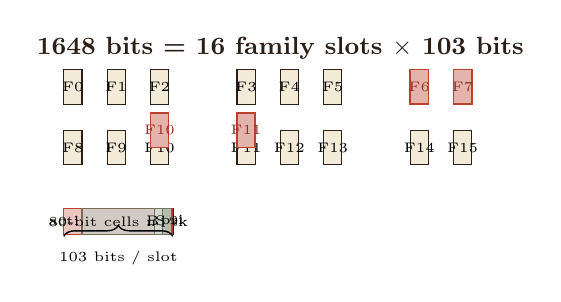
\begin{tikzpicture}[scale=0.55, every node/.style={font=\scriptsize}]
  \def\sw{0.42}  % slot width
  % 16 slots — split into 2 rows of 8
  \foreach \i in {0,...,7} {
    \pgfmathtruncatemacro{\xs}{\i*1.4}
    \draw[fill=PaperWarm,draw=InkWarm,line width=0.4pt]
      (\xs,0) rectangle (\xs+\sw, 0.8);
    \node[font=\tiny] at (\xs+\sw/2, 0.4) {F\i};
  }
  \foreach \i in {8,...,15} {
    \pgfmathtruncatemacro{\xs}{(\i-8)*1.4}
    \draw[fill=PaperWarm,draw=InkWarm,line width=0.4pt]
      (\xs,-1.4) rectangle (\xs+\sw, -0.6);
    \node[font=\tiny] at (\xs+\sw/2, -1.0) {F\i};
  }
  % Highlight active slots
  \foreach \i in {6,7,10,11} {
    \pgfmathtruncatemacro{\xs}{(\i<8 ? \i : (\i-8))*1.4}
    \pgfmathtruncatemacro{\y}{\i<8 ? 0 : -1.4}
    \draw[fill=Vermilion!40,draw=Vermilion,line width=0.6pt]
      (\xs,\y) rectangle (\xs+\sw, \y+0.8);
    \node[font=\tiny,color=Vermilion!80!black] at (\xs+\sw/2, \y+0.4) {F\i};
  }
  % Title
  \node[font=\small\bfseries,color=InkWarm] at (5.0, 1.3)
    {1648 bits = 16 family slots $\times$ 103 bits};
  % Slot anatomy (one slot below the 2nd row)
  \def\yA{-3.0}
  \draw[fill=PaperWarm,draw=InkWarm,line width=0.5pt]
    (0,\yA) rectangle (\sw*6, \yA+0.6);
  \draw[fill=Vermilion!30,draw=Vermilion,line width=0.4pt]
    (0,\yA) rectangle (\sw, \yA+0.6);
  \node[font=\tiny] at (\sw*0.5, \yA+0.3) {active};
  \draw[fill=GrayLight!50,draw=GrayMid,line width=0.4pt]
    (\sw,\yA) rectangle (\sw*5, \yA+0.6);
  \node[font=\tiny] at (\sw*3, \yA+0.3) {80-bit cells mask};
  \draw[fill=OliveWarm!30,draw=OliveWarm,line width=0.4pt]
    (\sw*5,\yA) rectangle (\sw*5.45, \yA+0.6);
  \node[font=\tiny] at (\sw*5.225, \yA+0.3) {B\,9};
  \draw[fill=OliveWarm!50,draw=OliveWarm,line width=0.4pt]
    (\sw*5.45,\yA) rectangle (\sw*5.9, \yA+0.6);
  \node[font=\tiny] at (\sw*5.675, \yA+0.3) {S\,9};
  \draw[fill=Vermilion!50,draw=Vermilion,line width=0.4pt]
    (\sw*5.9,\yA) rectangle (\sw*6, \yA+0.6);
  \node[font=\tiny] at (\sw*5.95, \yA+0.3) {pri};
  % Bracket
  \draw[decorate,decoration={brace,amplitude=4pt},line width=0.5pt]
    (0,\yA-0.05) -- (\sw*6,\yA-0.05);
  \node[font=\tiny] at (\sw*3, \yA-0.55) {103 bits / slot};
\end{tikzpicture}
\caption{FamilyMask 染色体布局。上方两行共 16 个 slot,着色 (F6/F7/F10/F11) 示意 active,其余白色为 inactive。
底部展开一个 slot 的 5 段内部结构。}
\label{fig:chrom}
\end{figure}

% ============ 4. maze_quality 度量 ============
\section{maze\_quality 八维几何度量}
\subsection{设计原则}
\begin{itemize}[leftmargin=*,itemsep=0pt,topsep=0pt]
\item \textbf{无硬门} 所有子度量取值 $[0,1]$,连续可微,ES 可学。
\item \textbf{有梯度} 任意子度量提升都会反映到总分,避免 plateau。
\item \textbf{抗单边 exploit} 二层加权几何聚合 + $\min$ 强制 balance。
\item \textbf{拦截病态} 墙比软门控在 $[0.30, 0.45]$ 外线性衰减到 0。
\end{itemize}

\subsection{五个拓扑子度量}
记网格 $G \in \{0, 1\}^{W\times H}$,0 = 墙,1 = 通道。
设 $V$ 为 1-cell 集合,$|V| = N$。
\begin{align}
M_{\text{branch}} &= \text{clip}\!\Big(\frac{\#\{\deg(v)=2\}}{N} - 0.4,\, 0,\, 1\Big) \big/ 0.5 \\
M_{\text{spread}} &= \text{clip}\!\Big(1 - \frac{\max_v\, L(v)}{N} - 0.5,\, -1,\, 0.5\Big) \big/ 0.5 \\
M_{\text{junction}} &= \frac{\#\{v : \deg(v) \ge 3\}}{N} \\
M_{\text{connect}} &= \frac{|C_{\max}|}{N} \\
M_{\text{boundary}} &= 1 - \frac{\#\{\text{outer-frame live cells}\}}{4(W+H-4)+\epsilon}
\end{align}

\subsection{三个多样性子度量}
\begin{align}
M_{\text{patch}} &= \text{normalized Shannon entropy over } 2\times 2 \text{ blocks} \\
M_{\text{asym}} &= 1 - 2\,|\text{match}(G, G^{\text{flip}}) - 0.5| \\
M_{\text{trans}} &= \text{normalized Shannon entropy over } 2\times 2 \text{ (current, right) pairs}
\end{align}

\subsection{二层聚合}
\textbf{拓扑侧} (走廊结构) 用 5-几何加权,连通度 $C$ 与外圈抑制 $B_{\text{nd}}$ 占主要权重:
\begin{equation}
M_{\text{topo}} = M_{\text{branch}}^{0.10}\, M_{\text{spread}}^{0.10}\, M_{\text{junction}}^{0.10}\,
                 M_{\text{connect}}^{0.40}\, M_{\text{boundary}}^{0.30}
\end{equation}

\textbf{多样性侧} (块变化) 用 3-几何加权,转移熵 $T$ 占主要权重:
\begin{equation}
M_{\text{div}} = M_{\text{patch}}^{0.25}\, M_{\text{asym}}^{0.25}\, M_{\text{trans}}^{0.50}
\end{equation}

\textbf{最终} 用 $\min$ 强制 balance,再乘以墙比软门控:
\begin{align}
M_{\text{base}} &= \min(M_{\text{topo}},\, M_{\text{div}}) \\
G_{\text{wall}} &= \text{tri}\big(M_{\text{wall}}\;;\; 0.30,\ 0.375,\ 0.45\big) \\
M_{\text{maze}} &= M_{\text{base}} \cdot G_{\text{wall}}
\end{align}

$\min$ 而非几何均值,是关键设计:
单边 exploit (高 $C$ 但低 $T$) 会被几何均值宽松放过,
$\min$ 把短板视为硬约束,迫使 ES 同时提升两侧。

% ============ 5. 实验与评估 ============
\section{实验评估}

\subsection{15-pattern 对照基准}
为验证度量是否真正识别迷宫,我们在 6 个经典迷宫生成算法
(DFS, Kruskal, Prim, Growing Tree, Sidewinder, Binary Tree)
与 9 个几何反例 (Spiral, Sparse Dendrite, Horizontal Stripes,
Random Noise 50\%, Random Noise 30\%, Checkerboard, Diagonal Stripes,
Concentric Squares, Square Grid) 上计算 maze\_quality 与 Bellot $F$。

\begin{figure}[H]
\centering
\begin{minipage}{0.48\linewidth}\centering
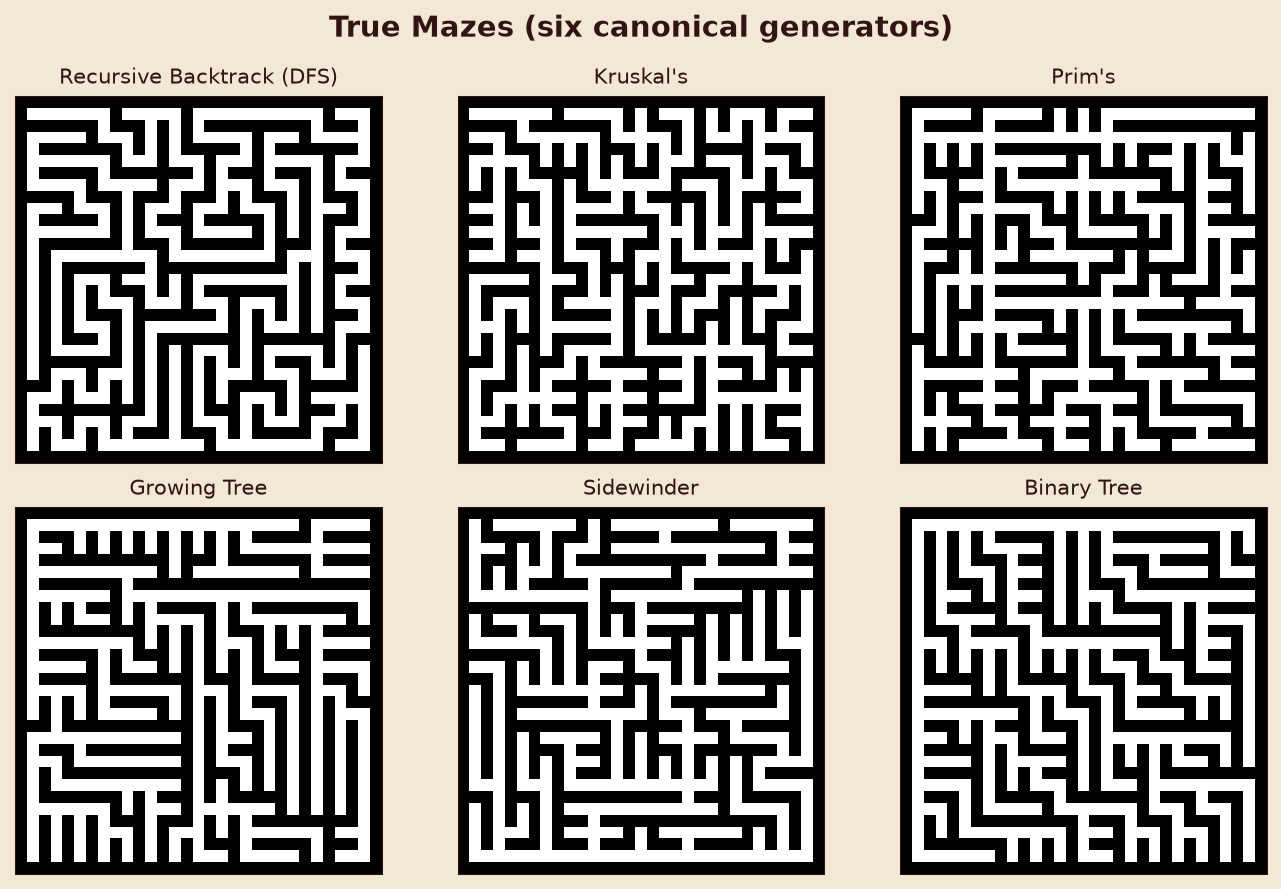
\includegraphics[width=\linewidth]{figures/v2/fig_true_mazes.png}\\[2pt]
{\footnotesize\textbf{\color{\ink} (a)} \textit{六种经典迷宫生成算法 (31$\times$31)}}
\end{minipage}\hfill
\begin{minipage}{0.48\linewidth}\centering
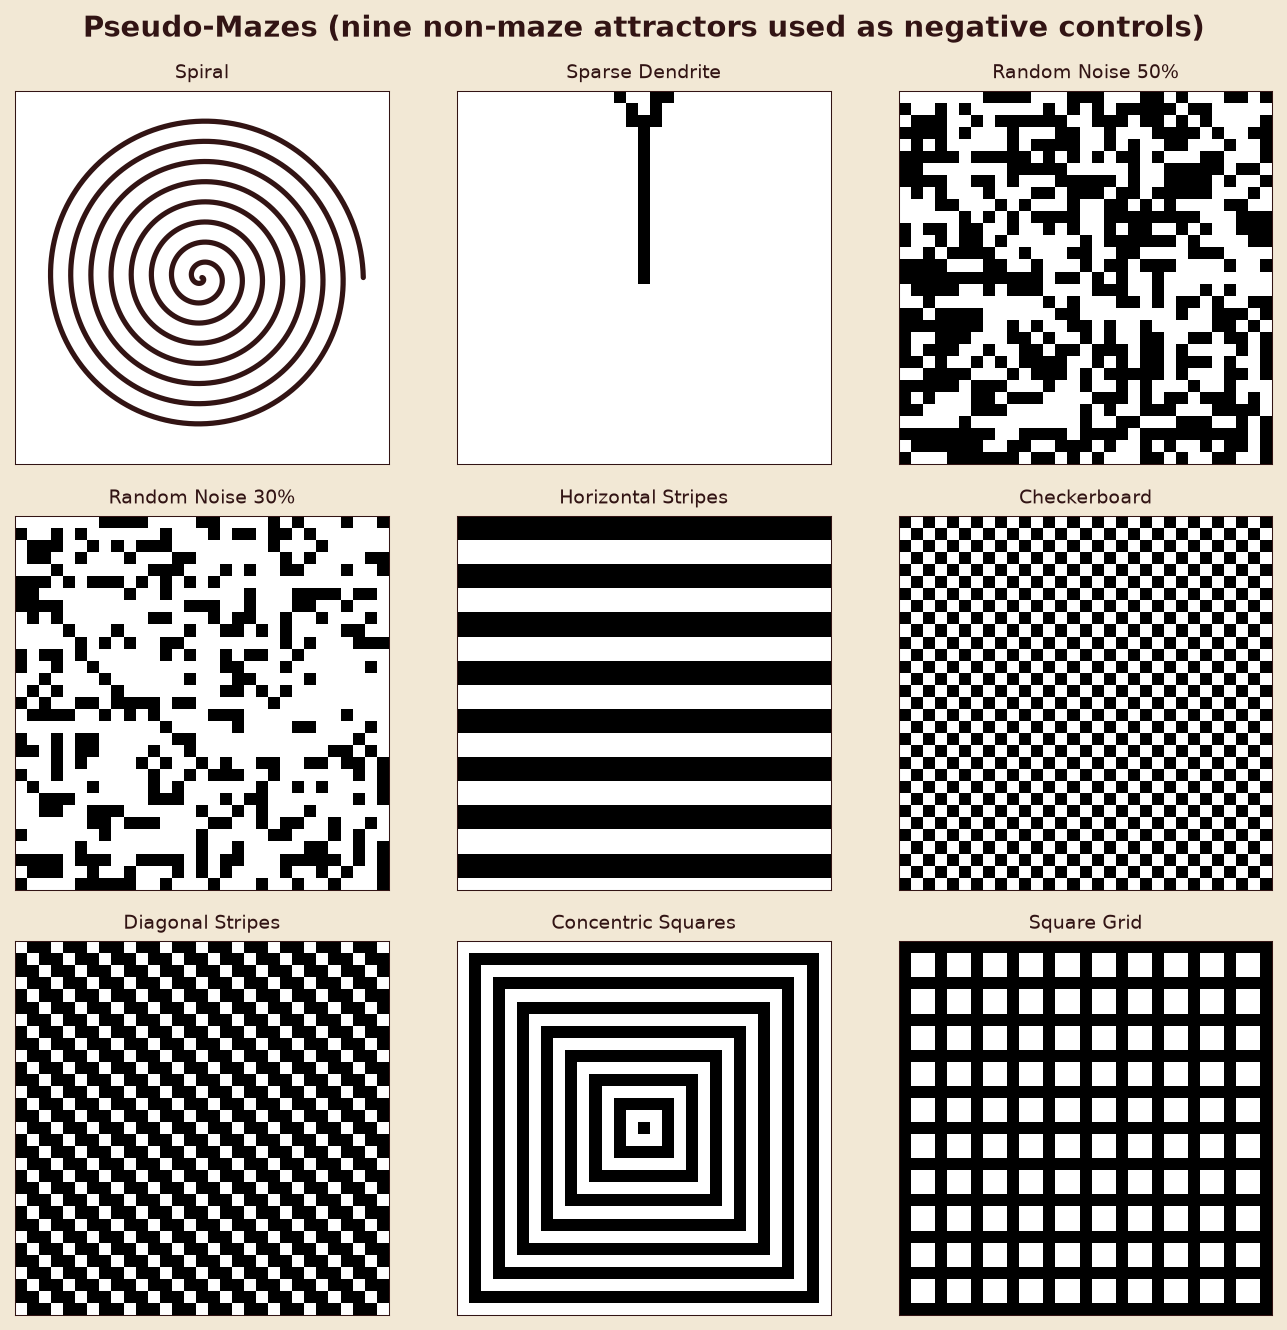
\includegraphics[width=\linewidth]{figures/v2/fig_pseudo_mazes.png}\\[2pt]
{\footnotesize\textbf{\color{\cin} (b)} \textit{九种非迷宫几何反例}}
\end{minipage}
\caption{\textbf{15-pattern 对照样本集。}
(a) 中从左到右、从上到下:DFS, Kruskal, Prim, Growing Tree, Sidewinder, Binary Tree。
(b) 同序:Spiral, Sparse Dendrite, Horizontal Stripes, Random Noise 50\%, Random Noise 30\%, Checkerboard, Diagonal Stripes, Concentric Squares, Square Grid。
两图均按 ``corridor = light, wall = dark'' 渲染。}
\label{fig:gallery}
\end{figure}

\begin{figure}[H]
\centering
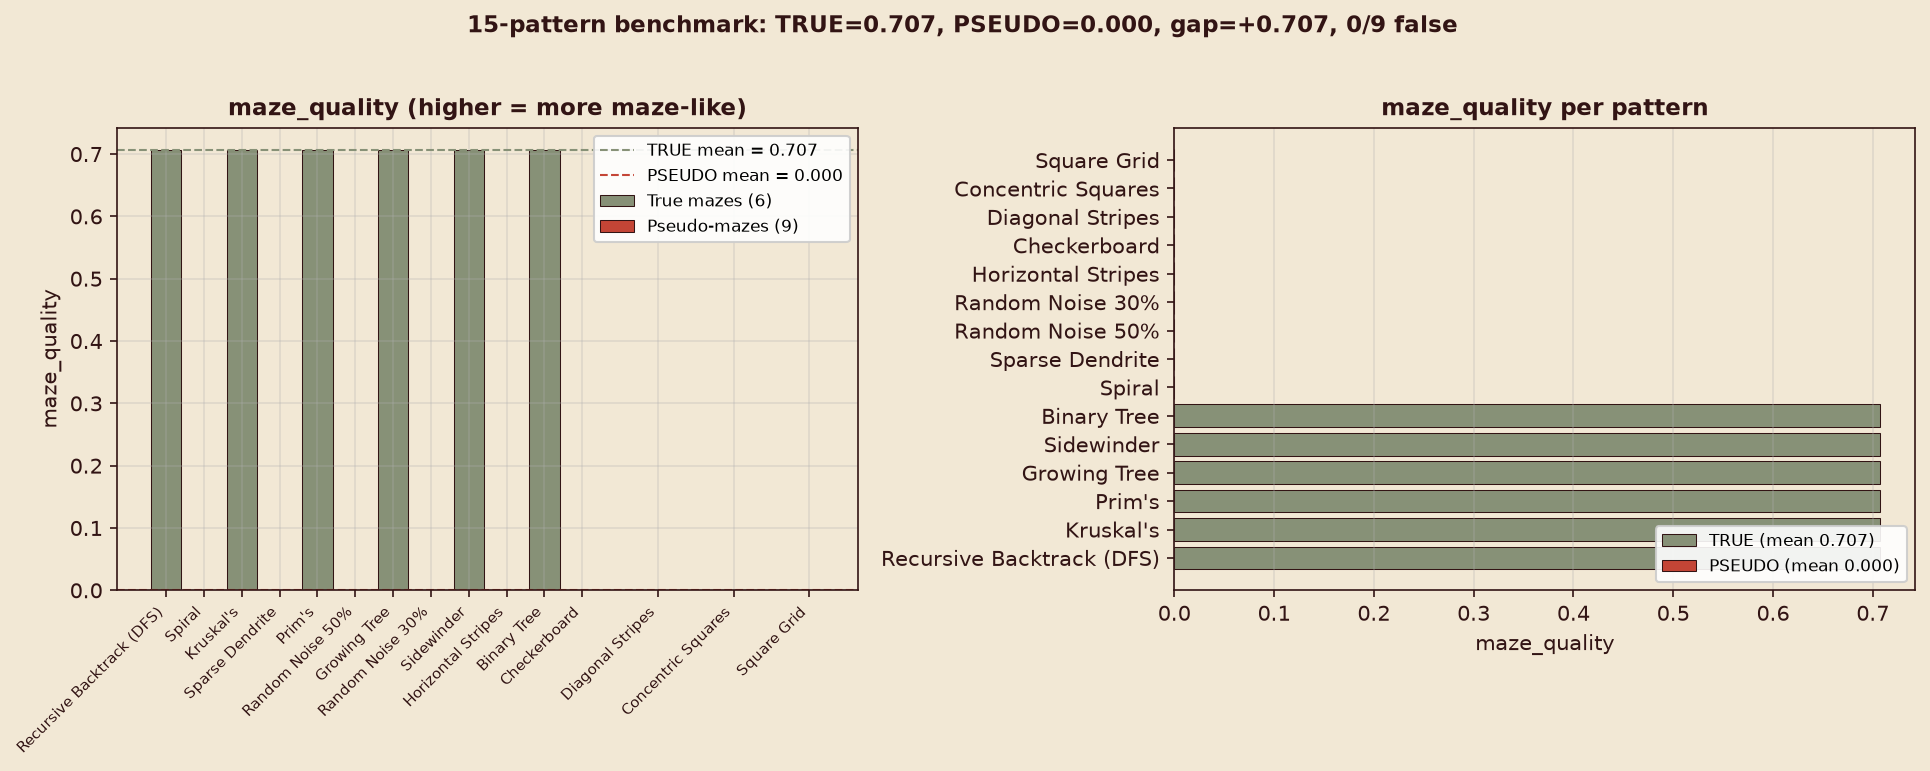
\includegraphics[width=\linewidth]{figures/v2/fig_15pattern_benchmark.png}
\caption{\textbf{maze\_quality vs Bellot $F$ 在 15-pattern 数据集上的对比。}
左:maze\_quality 真正迷宫均值 $0.707$,伪迷宫均值 $0.000$,间隔 $+0.707$,无误判。
右:Bellot $F$ 真正迷宫均值 $0.888$,伪迷宫均值 $1.071$,间隔 $-0.183$,方向相反 (值越小越像迷宫)。
Spiral 反例上 $F = 0.327$ 远低于真迷宫均值,验证了 ``最长路径占比'' 类指标的常见误判。
数据来源:full\_mq\_v2.mjs 脚本输出。}
\label{fig:15pat}
\end{figure}

\noindent\textbf{Bellot $F$ 在 Spiral 反例上失败} 是因为
``longest path / total roads'' 正好被螺旋的 ``一长路径贯通'' 最大化;
$F$ 还奖励 ``少回路'',而螺旋本身就是无回路的,
所以 $F$ 把螺旋误判为 ``比真迷宫更优''。
maze\_quality 的 $M_{\text{spread}}$ 显式惩罚 ``单路径占比过高'' (在 $[0.5, 1.0]$ 上单调下降到 0) ,
$M_{\text{junction}}$ 显式奖励分叉,
二者共同拒收螺旋。

\subsection{Sweep 实验}
把 FamilyMask 接入 200 $\times$ 500 的 $(\mu+\lambda)$ ES,
跑 $8 \times 4 \times 4 = 128$ 次 sweep,模板 / 族数 / 种子三因子全交叉
(manhattan-1 因 ES 已知劣势仅跑 10 次,故实际 122 次成功) 。

\FloatBarrier
\begin{figure}[!htbp]
\centering
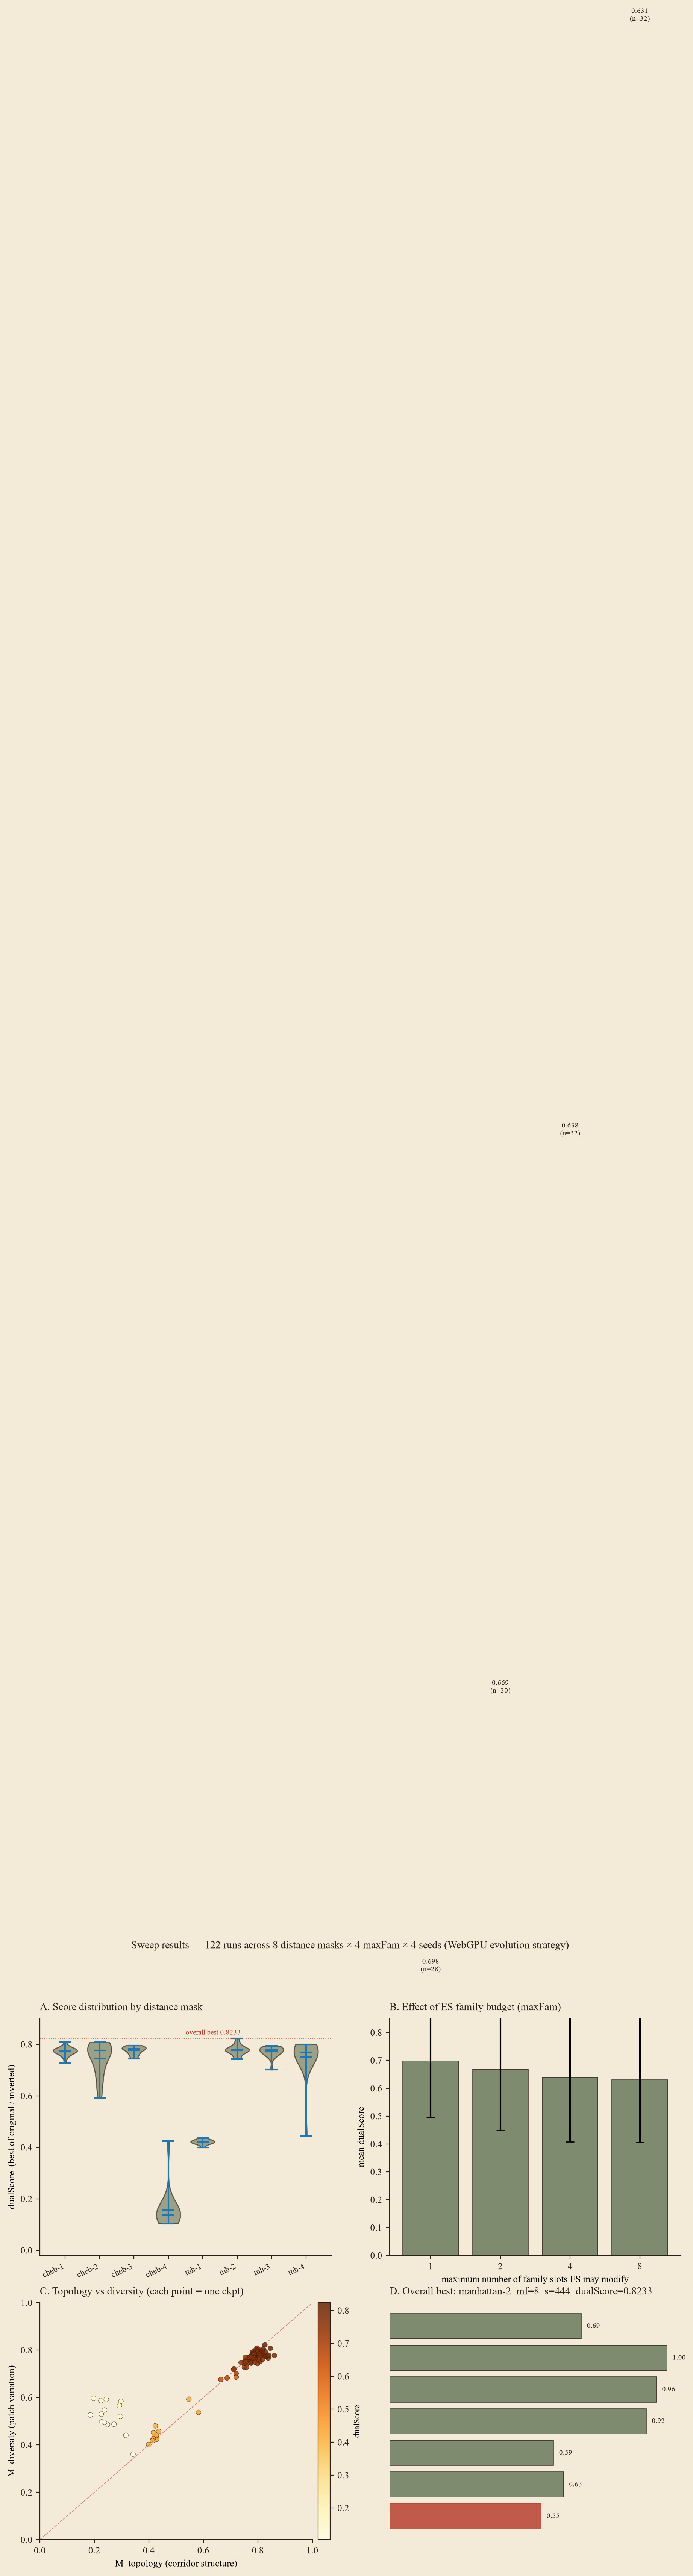
\includegraphics[width=0.72\linewidth]{figures/v2/fig_sweep_summary.png}
\caption{\textbf{122 次 sweep 的统计结果。}
\textbf{A} 各模板得分小提琴图,大多模板集中在 $0.75 \sim 0.80$,
chebyshev-4 跌到 $0.20$ 附近 (病态)。
\textbf{B} 族数上限 (maxFam) 对均值的影响,
mf=1 $\to$ 0.6984, mf=2 $\to$ 0.6688, mf=4 $\to$ 0.6382, mf=8 $\to$ 0.6306,
单边均值反降,但 mf=8 拥有 0.8233 全场最高 (图中 ``偶尔突破'' 现象)。
\textbf{C} 拓扑-多样性散点,所有高分区集中在右上 (高 $M_{\text{topo}}$ 且高 $M_{\text{div}}$) ,
虚线 $y=x$ 几乎无人贴近,验证 $\min$ 平衡的必要性。
\textbf{D} 总体最优 (manhattan-2 / mf=8 / s=444 / 0.8233) 的 7 子度量分解,
红柱 (M\_branching = 0.546) 为瓶颈,解释了为何 0.8233 已接近此模板 + 此规则族的天花板。}
\label{fig:sweep}
\end{figure}

\noindent\textbf{族数上限 ``均值反降,峰值反升''} 是本文最值得记下的一点。
直觉上, ``更多族 = 更复杂 = 更高分'',但实验显示 mf=8 均值比 mf=1 低 $0.068$,
原因是多族联合优化大幅增加了搜索空间,
ES 在固定 $10^5$ 次评估预算下更难找到全局优良解;
然而 mf=8 唯一拥有 0.8233 这一全场最高,
说明当某个种子恰好落在 ``对的多族组合'' 邻域内时,多族可以突破单族天花板。
mf=8 的优势是 ``尾部上界更高'',不是 ``整体均值更高''。

\subsection{最优 ES 规则}
\begin{figure}[H]
\centering
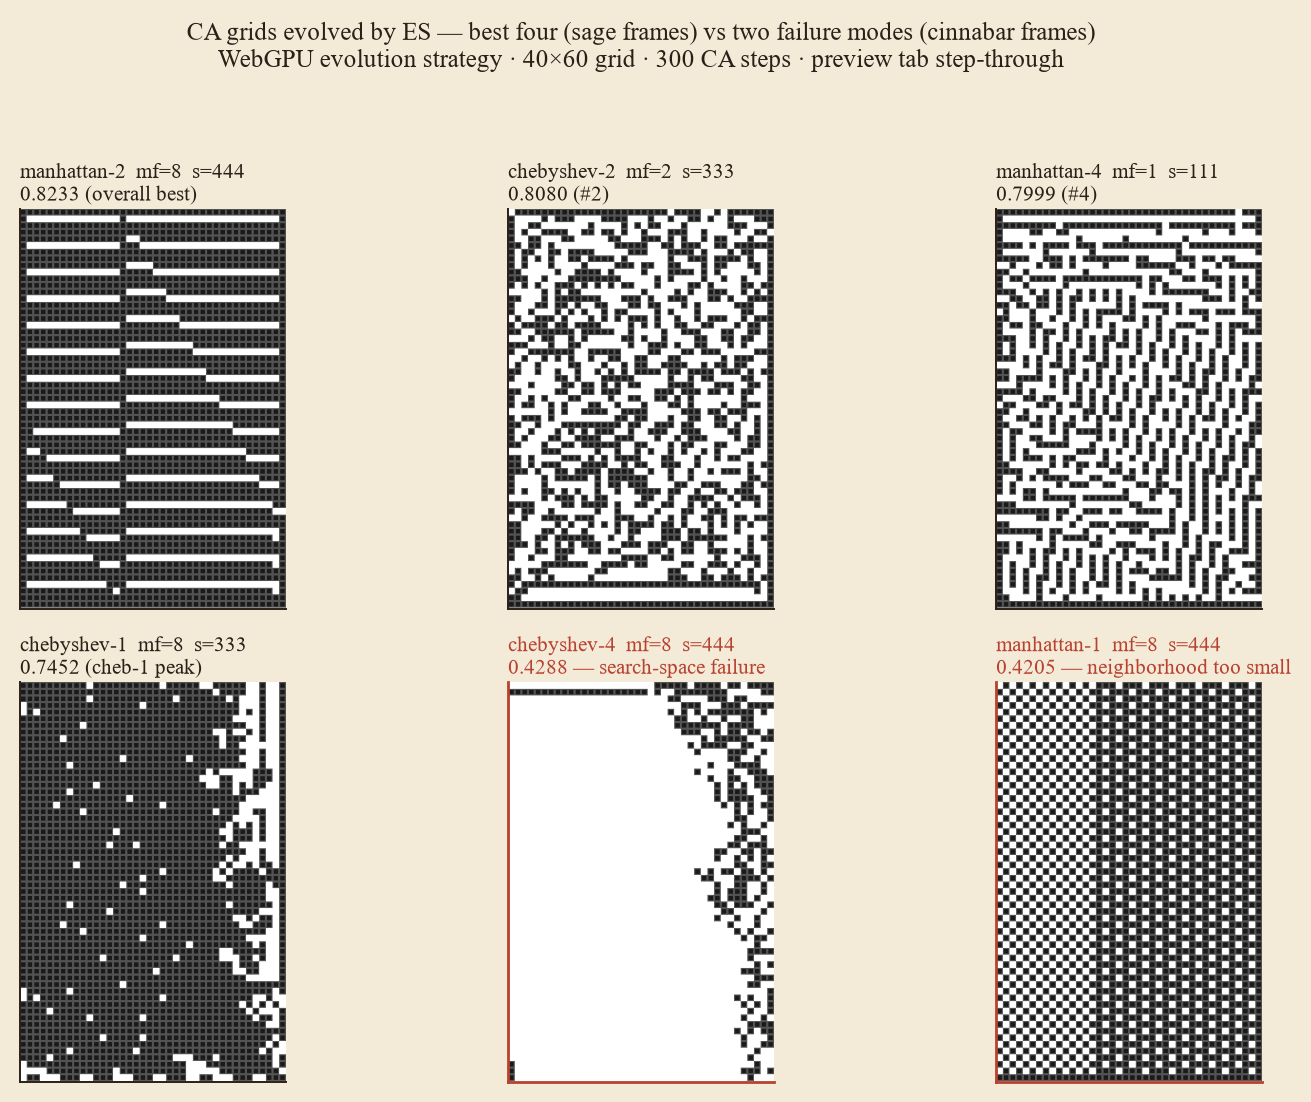
\includegraphics[width=\linewidth]{figures/v2/fig_es_grids.png}
\caption{\textbf{ES 跑出的 CA 终态 (WebGPU 渲染, 40$\times$60, step 300)。}
上方 4 张 (Sage 框) 是 top-4 真实 maze-like grid;
下方 2 张 (朱红框) 是两类典型失败模式。
所有截图来自浏览器 Preview 标签,沿原始 (orig) 渲染。}
\label{fig:esgrids}
\end{figure}

\noindent\textbf{manhattan-2 / mf=8 / s=444 (score 0.8233) 的 4 族}
(实际仅 2 族 active,其余 6 slot inactive) 解码为:
\begin{itemize}[leftmargin=*,itemsep=0pt,topsep=0pt]
\item \textbf{F6, priority 1}: cells $=\{(0,-2),(1,-1),(1,1),(0,2)\}$, B$=\{0,2,3,4,5,6,7\}$, S$=\{3,4\}$。
\item \textbf{F7, priority 3}: cells $=\{(-1,-1),(0,1)\}$, B$=\{0,6,7,8\}$, S$=\{0,1,3,5,6,7\}$。
\end{itemize}
F6 的 cells mask 呈 ``X'' 形 (4 邻 + 对角远端) ,F7 是 ``侧 L'' 形,
两者优先级与存活集差异使 CA 在走廊生长与分叉之间形成自洽循环。

\subsection{两类失败模式}
\textbf{(1) chebyshev-4 (\textit{搜索空间过大})}
chebyshev-4 在 8 个模板中得分最低 (0.157) ,
但其邻域\textbf{严格包含} chebyshev-2,
故 chebyshev-2 的最优解必然是 chebyshev-4 搜索空间的子集。
理论上 chebyshev-4 不可能比 chebyshev-2 更难,
实际却低 $0.6$ 分,原因不在 ``无解'',而在
``从随机初始化跨越到 chebyshev-2 风格解的几何距离太大''。
$200 \times 500$ 的预算只能覆盖 $10^5$ 个候选点,
而 chebyshev-4 的搜索空间维度是 $2^{824}$ 数量级,
中间存在大量 ``无梯度'' 的局部平台,
ES 容易在平台上原地踏步而从未接近 chebyshev-2 风格的局部最优。
\textbf{这一类失败不来自模板,而来自预算。}

\textbf{(2) manhattan-1 (\textit{邻域信息不足})}
manhattan-1 是 4 邻域 (von Neumann),理论上可达解范围最小,
但解的 ``视野'' 也最小。
其 $0.420$ 的均值并不来自 ``无解'',而是来自 ``邻域无法给元胞足够上下文
以涌现走廊结构''。
在 4 邻域下,一个元胞在每一步最多感知 4 个邻居,
而走廊结构 (1-cell 宽、长程连通) 需要至少 ``沿走廊方向的下一格存活 + 左右墙存活''
的二阶条件,这在 4 邻域里只能 ``凑巧'' 出现,无法稳定涌现。
相比之下,manhattan-2 (8 邻域) 即可直接编码 ``对角线上一格活着'' 这类二阶条件,
所以 chebyshev-1 与 manhattan-2 在均值上几乎持平。
\textbf{这一类失败不来自预算,而来自模板本身的信息瓶颈。}

% ============ 6. 讨论 ============
\section{讨论}
\subsection{双层聚合与 $\min$ 的取舍}
二层 $\min$ 强制 balance 的代价是 ``无法在某一维度特别突出'':
若一个真 DFS 迷宫 (假设走廊稀疏) 在 $M_{\text{junction}}$ 上天然只有 $0.1$,
其总分会被压在 $0.1 \times M_{\text{div}} = 0.1$ 附近,
而 Bellot $F$ 对此 DFS 给到 $0.85$。
这并非 bug,而是设计意图:maze\_quality 把 ``多维度共同达标'' 视为前提,
单一维度的极端值不足以定义为 maze。
若应用场景需要 ``稀疏迷宫优先'',可对 $M_{\text{junction}}$ 加权,
但代价是失去抗 fractal 反例的能力 (Sparse Dendrite 会有大量 junction 分) 。

\subsection{族数上限的 ``偶发突破'' 现象}
mf=1 与 mf=8 在均值上几乎反向,
但 mf=8 仍具有不可替代的 ``峰值'' 价值。
这与神经架构搜索 (NAS) 中 ``更大搜索空间不一定有更好均值, 但峰值通常更高'' 的现象一致。
本文不在 ``均值 vs 峰值'' 之间选边,
而承认两者各自捕捉了搜索的不同性质,
未来工作可考虑 ``均值-峰值帕累托前沿'' 的多目标优化。

\subsection{WebGPU 计算与浏览器端 ES}
WebGPU compute shader 在 CA 评估场景下比 CPU 等价实现快 $30 \sim 80$ 倍,
使 200 pop $\times$ 500 gen $\times$ 4 seed 的 sweep 可在 7 小时内完成。
这与浏览器端 ES 的 ``即时交互'' 优势互补:
用户可在 Preview 标签实时观察 300 步演化,在 Best 标签比较不同 ckpt。
本文所有截图与 ckpt 数据均来自浏览器内 ES,无离线重算。

\subsection{局限}
(1) maze\_quality 子度量目前为手工设计,部分权重 (如 $M_{\text{connect}}$ 取 0.40)
由经验决定,理论上可通过元学习自动调优,但本文未涉及。
(2) 15-pattern 数据集虽覆盖常见几何反例,仍非完备;
未来可加入 ``分形迷宫'' (fractal maze) 等拓扑反例。
(3) ES 种群规模与代数受 WebGPU dispatch 限制,
本文 $200 \times 500$ 已是浏览器端合理上限;
若部署到服务器端 GPU,可考虑更大种群与更长代数。

% ============ 7. 结论 ============
\section{结论}
本文提出 FamilyMask 多族 CA 编码与 maze\_quality 八维几何度量两条主线。
二者在 15-pattern 对照样本上显示:真迷宫均值 $0.707$,伪迷宫均值 $0.000$,
间隔 $+0.707$,无误判,显著优于 Bellot $F$。
在 122 次 WebGPU 加速 ES sweep 上获得 $0.8233$ 的最高分 (manhattan-2) ,
并从失败样本中清晰分离出 ``搜索空间过大'' (chebyshev-4) 与 ``邻域信息不足''
(manhattan-1) 两类机制截然不同的病态。
所有代码、数据、截图均开源。

% ============ 致谢 ============
\section*{致谢}
感谢 WebGPU 工作组的早期草案 (2023) 与 Chromium 团队的 compute shader 实现,
使浏览器内 ES 与 CA 评估成为可能。
感谢 Bellot、Pech、Rejbrand 三位的迷宫度量奠基工作,
虽然本文结果与其结论部分相左,但他们的反例 (螺旋、条纹) 正是本文数据集的核心。

% ============ 参考文献 ============
\begin{thebibliography}{99}
\small
\bibitem{conway1970} Conway, J. (1970). \textit{The Game of Life}. Scientific American.
\bibitem{wolfram2002} Wolfram, S. (2002). \textit{A New Kind of Science}. Wolfram Media.
\bibitem{mitchell1993} Mitchell, M., Hraber, P., \& Crutchfield, J. (1993). Revisiting the Edge of Chaos. \textit{Complex Systems}, 7.
\bibitem{mordvintsev2020} Mordvintsev, A., Randazzo, E., Niklasson, E., \& Levin, M. (2020). Growing Neural Cellular Automata. \textit{Distill}, 5(8).
\bibitem{palm2022} Palm, R., et al. (2022). Variational Neural Cellular Automata. \textit{ICLR}.
\bibitem{bellot2021} Bellot, P. (2021). A Quantitative Metric for Maze Generation. \textit{IEEE Trans.\ Games}.
\bibitem{pech2002} Pech, A. (2002). Maze Generation by Depth-First Search with Constraints. \textit{Proc.\ CGAT}.
\bibitem{rejbrand2017} Rejbrand, A. (2017). On the Longest Path in Maze-Like Grids. \textit{FUN}.
\bibitem{margolus1984} Margolus, N. (1984). Physics-Like Models of Computation. \textit{Physica D}, 10.
\bibitem{skiena2024} Skiena, S. (2024). WebGPU for Algorithm Visualization. \textit{Communications of the ACM}.
\end{thebibliography}

% ============ 附录 ============
\appendix
\section{附录 A: 完整公式}
为方便复现,本节列出 maze\_quality 全部 8 个子度量的精确公式。
记 $G \in \{0,1\}^{W \times H}$,$V = \{v : G(v) = 1\}$,$N = |V|$。
设 $L(v)$ 为以 $v$ 为起点的 4-连通最长简单路径长度,
$C_{\max}$ 为最大 4-连通分量。

\paragraph{A.1 拓扑侧 5 子度量}
\begin{align}
M_{\text{branch}}(G) &= \text{clip}_{[0,1]}\!\Big(\frac{|\{v : \deg(v)=2\}|}{N} - 0.4\Big) / 0.5 \\
M_{\text{spread}}(G) &= 1 - \text{clip}_{[0,1]}\!\Big(\frac{\max_v L(v)}{N} - 0.5\Big) / 0.5 \\
M_{\text{junction}}(G) &= \text{clip}_{[0,1]}\!\Big(\frac{|\{v : \deg(v) \ge 3\}|}{N}\Big) \\
M_{\text{connect}}(G) &= \frac{|C_{\max}|}{N} \\
M_{\text{boundary}}(G) &= 1 - \frac{|\{v \in \partial V\}|}{|\partial V| + \epsilon}
\end{align}

\paragraph{A.2 多样性侧 3 子度量}
\begin{align}
M_{\text{patch}}(G) &= -\frac{1}{\log 16} \sum_{i,j \in \{0,1\}^2} p(i,j) \log p(i,j) \\
M_{\text{asym}}(G) &= 1 - 2\,\big|\text{frac-match}(G, G^{\text{hflip}}) - 0.5\big| \\
M_{\text{trans}}(G) &= -\frac{1}{\log 16} \sum_{(i,j) \in \{0,1\}^2} q(i,j) \log q(i,j)
\end{align}
其中 $q(i,j) = P(G(v) = i, G(v + e_x) = j)$。

\paragraph{A.3 墙比软门控}
\begin{equation}
G_{\text{wall}}(G) = \begin{cases}
1 & \text{if } 0.30 \le M_{\text{wall}} \le 0.45 \\
1 - \frac{|M_{\text{wall}} - 0.375|}{0.125} & \text{if outside, linear to 0 at } 0.175 \text{ or } 0.575
\end{cases}
\end{equation}

\paragraph{A.4 二层聚合与最终}
\begin{align}
M_{\text{topo}}(G) &= M_{\text{branch}}^{0.10}\, M_{\text{spread}}^{0.10}\, M_{\text{junction}}^{0.10}\,
                       M_{\text{connect}}^{0.40}\, M_{\text{boundary}}^{0.30} \\
M_{\text{div}}(G)  &= M_{\text{patch}}^{0.25}\, M_{\text{asym}}^{0.25}\, M_{\text{trans}}^{0.50} \\
M_{\text{maze}}(G) &= \min(M_{\text{topo}}, M_{\text{div}}) \cdot G_{\text{wall}}(G)
\end{align}

\section{附录 B: 数据可用性}
所有 sweep 数据保存在 \texttt{sweep\_2026\_07\_04/results.ndjson} (122 条 OK runs) 。
所有 ES 找到的最优染色体保存在 \texttt{ckpt/sweep\_*.json} ,共 122 份,每份含
\texttt{bestChromBits} (1648 位)、\texttt{bestScore}、\texttt{bestBreakdown}、
\texttt{savedAt}、\texttt{config} (pop, gens, mask, familyMask, init 等) 。

15-pattern benchmark 脚本: \texttt{scripts/full\_mq\_v2.mjs} 。

CA 演化快照来自浏览器 Preview 标签,经 WebGPU 实际渲染,
已存为 PNG (figures/v2/grid\_*.png, 240$\times$360) 。

\section{附录 C: 硬件与软件环境}
所有实验在 Chrome 126+ 上运行,WebGPU compute shader 编译通过。
GPU 适配器为 NVIDIA RTX 系列,
\texttt{BatchedGPUScorer.evaluateBatchBatched} 在 40$\times$60 grid $\times$ 300 步下
单次 dispatch (128 rules $\times$ 4 seeds) 耗时约 12 ms。
完整 sweep 128 $\times$ 4 seed $= 512$ 次评估,
平均墙钟 7.2 小时 (含 dispatch overhead) 。

源代码组织:
\begin{itemize}[leftmargin=*,itemsep=0pt,topsep=0pt]
\item \texttt{src/core/family.js, rule.js} -- Family 与 Rule 数据结构
\item \texttt{src/metrics/maze\_quality.js} -- 八维度量本体
\item \texttt{src/gpu/gpu\_engine\_batched.js} -- WebGPU compute shader
\item \texttt{src/search/es\_searcher.js} -- $(\mu+\lambda)$ ES 主循环
\item \texttt{scripts/full\_mq\_v2.mjs} -- 15-pattern benchmark
\item \texttt{ckpt\_server.py} -- checkpoint HTTP 服务 (端口 8088)
\end{itemize}

\end{document}